
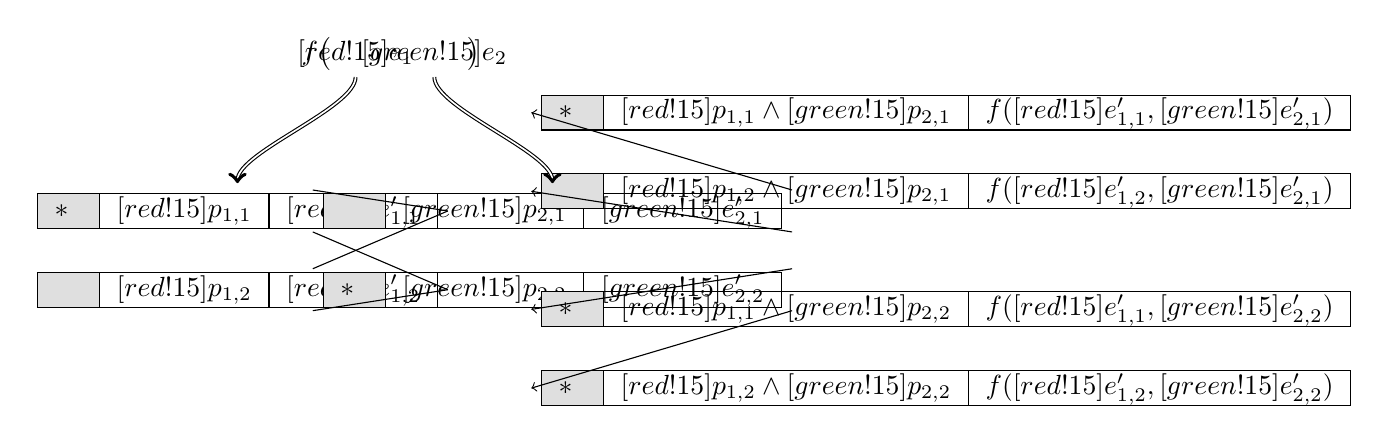
\begin{tikzpicture}[x=10mm, y=10mm]
\node      at (1, 5) {$f\big($};
\node (e1) at (1.5, 5) {$\highlight[red!15]{e_1}$};
\node      at (2, 5) {$,$};
\node (e2) at (2.5, 5) {$\highlight[green!15]{e_2}$};
\node      at (3, 5) {$\big)$};

\node (e11) at (0, 3) { 
    \begin{tabular}{|p{1em}|r|c|}\hline
    \cellcolor{gray!25} $\ast$ & $\highlight[red!15]{p_{1,1}}$ & $\highlight[red!15]{e'_{1,1}}$\\\hline
    \end{tabular}
};
\node (e12) at (0, 2) { 
    \begin{tabular}{|p{1em}|r|c|}\hline
    \cellcolor{gray!25}  & $\highlight[red!15]{p_{1,2}}$ & $\highlight[red!15]{e'_{1,2}}$\\\hline
    \end{tabular}
};

\node (e21) at (4, 3) { 
    \begin{tabular}{|p{1em}|r|c|}\hline
    \cellcolor{gray!25}  & $\highlight[green!15]{p_{2,1}}$ & $\highlight[green!15]{e'_{2,1}}$\\\hline
    \end{tabular}
};
\node (e22) at (4, 2) { 
    \begin{tabular}{|p{1em}|r|c|}\hline
    \cellcolor{gray!25}$\ast$ & $\highlight[green!15]{p_{2,2}}$ & $\highlight[green!15]{e'_{2,2}}$\\\hline
    \end{tabular}
};

\node (r1) at (9, 4.25) { 
    \begin{tabular}{|p{1em}|r|c|}\hline
    \cellcolor{gray!25} $\ast$ & $\highlight[red!15]{p_{1,1}} \land \highlight[green!15]{p_{2,1}}$ & $f(\highlight[red!15]{e'_{1,1}}, \highlight[green!15]{e'_{2,1}})$\\\hline
    \end{tabular}
};
\node (r2) at (9, 3.25) { 
    \begin{tabular}{|p{1em}|r|c|}\hline
    \cellcolor{gray!25}  & $\highlight[red!15]{p_{1,2}} \land \highlight[green!15]{p_{2,1}}$ & $f(\highlight[red!15]{e'_{1,2}}, \highlight[green!15]{e'_{2,1}})$\\\hline
    \end{tabular}
};

\node (r3) at (9, 1.75) { 
    \begin{tabular}{|p{1em}|r|c|}\hline
    \cellcolor{gray!25} $\ast$ & $\highlight[red!15]{p_{1,1}} \land \highlight[green!15]{p_{2,2}}$ & $f(\highlight[red!15]{e'_{1,1}}, \highlight[green!15]{e'_{2,2}})$\\\hline
    \end{tabular}
};
\node (r4) at (9, 0.75) { 
    \begin{tabular}{|p{1em}|r|c|}\hline
    \cellcolor{gray!25} $\ast$ & $\highlight[red!15]{p_{1,2}} \land \highlight[green!15]{p_{2,2}}$ & $f(\highlight[red!15]{e'_{1,2}}, \highlight[green!15]{e'_{2,2}})$\\\hline
    \end{tabular}
};
\draw[->, double, out=270, in=90, looseness = 0.5] (e1.south) to (e11);
\draw[->, double, out=270, in=90, looseness = 0.5] (e2.south) to (e21);

\draw (e11.east) -- (e21.175);
\draw (e11.east) -- (e22.175);
\draw (e12.east) -- (e21.185);
\draw (e12.east) -- (e22.185);

\draw[->] (e21.5) -- (r1.west);
\draw[->] (e21.355) -- (r2.west);
\draw[->] (e22.5) -- (r3.west);
\draw[->] (e22.355) -- (r4.west);
\end{tikzpicture}
